\section{General description}

\subsection{Product perspective}
 %Describes the environment of the system

\subsubsection{Description}
This is a new product which can be used in conjunction with any mobile text manipulation service, be this provided by the operating system or another application, capable of using the basic GSM character set, should you require encryption and decryption functionality.
\vspace{12pt}\\
The GSM character set only contains certain characters which limits which encryption methods we can make use of. Many encryption algorithms greatly increase the number of characters, but this approach will be infeasable.
\vspace{12pt}\\
Software interface - The software interface will make use of operating system features such as a clipboard on the device to facilitate copying and pasting of messages or ciphertexts.
\vspace{12pt}\\
User interface - The user interface is what will allow the user to encrypt a message and decrypt a message which has been sent by other users of this application.
\vspace{12pt}\\
Hardware Interface - The software will run on a mobile device that allows user interaction.


%Note:
%Required : Functionality must be provided if service is provided
%Extends : Extended functionality which can be provided, but not always.
\newpage
\subsubsection{Use Cases}
SMSEncryption Use case diagram

\begin{center}
 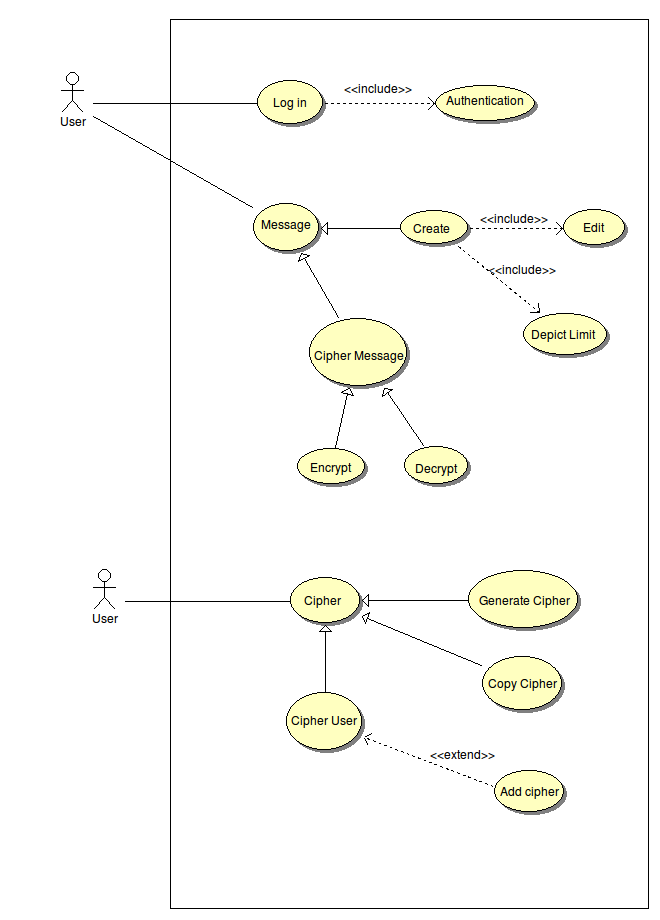
\includegraphics[width=13cm]{diagrams/UseCaseDiagrams/UseCaseSMSEncryption.png}
\end{center}




\subsection{Product features}
%An overview of the system's main features
%? complete list of "brief" use-case descriptions
%? features will be specified in detail in Section 3
\subsubsection{Log In}
\begin{itemize}
\item On first use a password must be created for future use by the user of the application.
\item The application will ask the user for login details which he/she must then enter correctly. 
\item If it is incorrect, the application will close preventing access for an unauthorised user.
\end{itemize}
\subsubsection{Message}
\textbf{Create}
\begin{itemize}
\item The plaintext is created independently by the user and input into the application
\item The plaintext can be created and edited within the application.
\end{itemize}
\textbf{Cipher Message}
\begin{itemize}
\item The user will select a relevant contact, that contacts details will then be used to perform encryption or decryption.\item The message will be encrypted to obtain the cipher text which the user can then copy out and send to the desired receiver via any messaging method.
\item The desired receiver will be able to decrypt the message into its plaintext.
\end{itemize}

\subsubsection{Device Synchronization}
\begin{itemize}
\item In order for communication to take place between two devices they need to be synchronized.
\item A user adds what is called a contact, it will ask the name of the contact as well as generate a unique word to be provided to the other person and an input box where the unique word appearing on the contacts phone.
\item Both users must add each other at the same time, because they need each other unique word that will be generated for their communication. This will synchronize communication between the devices.
\end{itemize}

\subsection{User characteristics}
%Assumptions about the users, their background, how
%much training they will need
%? e.g., different user interfaces for expert vs. novice users
%? Only user characteristics that affect the software
%requirements
\begin{itemize}
\item There will be only one user class who will have full access to all the features provided by the application after local authentication.
\item It is assumed that the user has proficient knowledge on how to copy items from messages such as SMS and paste it within this application.
\item Assumed that the users performed the device synchronization phase correctly as there is no way for the device to know.
\end{itemize}


\subsection{Constraints}
%Anything that will limit the designer's options
\begin{itemize}
\item The application must make use of the basic GSM character set.
\end{itemize}



\subsection{Assumptions and dependencies}
%List any assumed factors (as opposed to known facts) 
%that could affect the requirements stated in the SRS. 

\begin{itemize}
\item It is assumed that the amount of characters in the basic GSM character set is 128 for the 7-bit encoding used in GSM.
\item It is assumed that the devices being used allows for copy and pasting of text between different interfaces and applicaitons.
\end{itemize}
